\chapter{O problema e os seus desafios}
\label{cap_problema}


Neste capítulo, é feita uma síntese dos desafios do problema e uma discussão sobre a solução desenhada até ao momento para concretizar os objetivos definidos.

\section{Desafios}

No capítulo \ref{cap_estado_arte}, realizou-se um estudo abrangente sobre o estado da arte no que toca a projetos que utilizem \acrshort{ocr} e trabalhos relacionados com os objetivos listados para este projeto (\ref{section_objetivos}).  Através deste estudo, foi possível extrair um leque de problemas detetados na utilização de reconhecimento de texto em documentos, de forma generalizada ou para tipos específicos como é o caso deste trabalho. Em suma, os principais desafios são:
\begin{itemize}
    \item \textbf{Problemas de imagem} : tanto na imagem de input, como no documento original. Ex.: ruído, baixa resolução, má iluminação.
    \item \textbf{Problemas de reconhecimento} : estes são muitas vezes derivados do conjunto anterior, mas outras questões como léxico no documento desconhecido pelo motor OCR ou estruturas complexas podem provocar erros no reconhecimento.
    \item \textbf{Problemas nos resultados} : consideremos estes os problemas sobre as entidades reconhecidas pelo software, tanto o texto que em muitos casos apresenta erros como os próprios contentores em que estes são incluídos.
    \item \textbf{Problemas na extração de conteúdo} : no processo de criação de output, por vezes questões como a ordem de leitura dos blocos identificados, ou reposição de elementos não texto têm de ser abordados.
    \item \textbf{Validação da implementação} : de forma a verificar a eficácia da solução criada, geralmente datasets de teste e casos de estudo relevantes têm de ser criados.
\end{itemize}


\section{Plano da Solução}
\begin{wrapfigure}{r}{0.3\textwidth}
    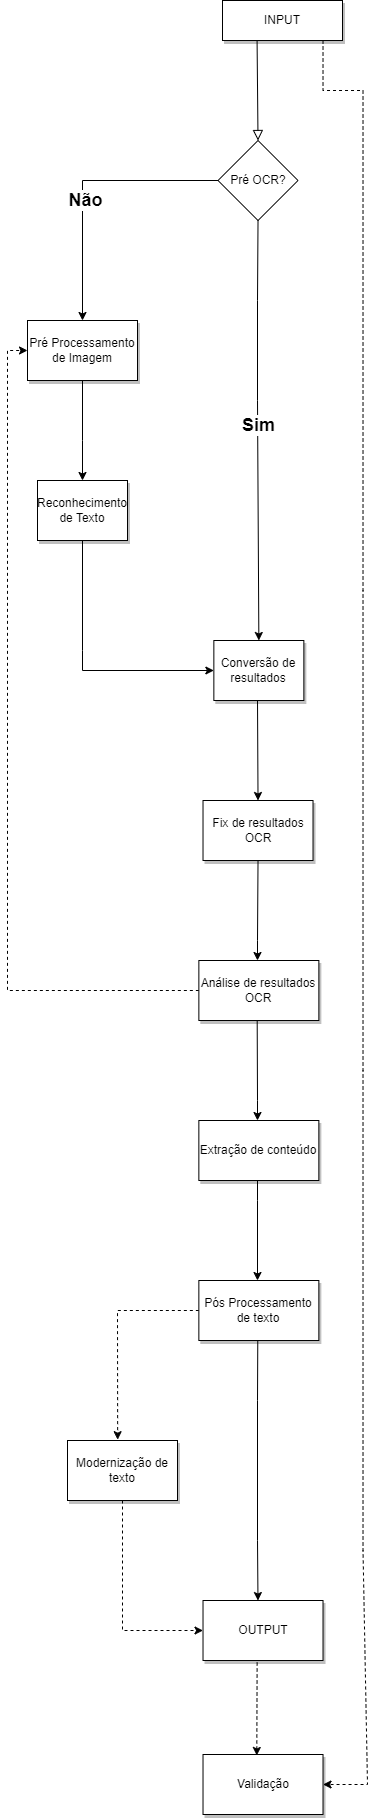
\includegraphics[width=0.25\textwidth]{images//diagramas/pipeline_geral.png}
    \caption{Pipeline da solução}
    \label{fig:pipeline_geral}
\end{wrapfigure}
Durante o estudo do estado da arte, tornou-se evidente que a maioria dos trabalhos com vista em extrair ou corrigir a extração de documentos utilizando reconhecimento de texto, de forma a manter o conteúdo e lógica original, seguem uma metodologia semelhante: uma primeira fase de pré processamento da imagem de input; possível segmentação da imagem entre texto e não texto; reconhecimento de texto; pós processamento do texto; possível pós processamento para segmentação de conteúdo específico de um tipo de ficheiro, como artigos, ou para reorganização dos resultados (ordem de leitura); criação de output.

Partindo desta base, a figura \ref{fig:pipeline_geral} representa o fluxo da solução planeada atualmente. 

A pipeline começa com a introdução de um input, podendo este ser sujeito de reconhecimento de texto, no caso de ser uma imagem, ou já possuir os resultados de reconhecimento, como hOCR. No caso de uma imagem, antes de ser aplicado o software de OCR, será realizado pré processamento da imagem para aumentar a chance de bons resultados de OCR.

Os resultados de OCR são então convertidos para uma estrutura de dados genérica, de modo a englobar os diferentes tipos de resultados possíveis de diferentes tipos de ficheiros ou motores de OCR. Em diante, esta estrutura será usada nos módulos que utilizam os resultados de OCR.

Depois, passa-se por um processo de pós processamento básico dos resultados de OCR. Tal tem o intuito de corrigir erros menos severos no que toca às \textit{bounding boxes} dos resultados e lixo reconhecido pelo motor.

Uma análise dos resultados limpos é então realizada, extraindo informação sobre o texto reconhecido, estimas do possível layout, erros de reconhecimento, etc.. Com os resultados da análise feita, abre-se a possibilidade de realizar um tratamento de imagem diferente dedicado à resolução de problemas detetados, por exemplo: detetado um \acrshort{dpi} de imagem muito baixo, este é um indicador de que a resolução da imagem poderia ser aumentado para melhorar o reconhecimento, procedimento comum no estudo feito.

Utilizando os resultados da análise, são de pois aplicados algoritmos para extração do conteúdo do documento. Aqui o principal objetivo será o cálculo da ordem de leitura e agrupamento dos elementos em conjuntos como artigos.
Além disso, o objetivo secundário envolvente da modernização de texto poderá nesta etapa ser aplicado.

Finalmente, o output final é gerado. Diferentes formas de output serão disponibilizadas dependendo da estrutura pretendida, por exemplo: markdown ou texto simples no caso de apenas se querer os elementos do texto isolado; html para reconstruir a estrutura do documento original. 

